% 依据固定来源 PDF 第 2 页半椭圆、梯形及两处 2r 尺寸标注重绘
% source_id=src-3612a22ce3848ad6ebbec4d94861dd64b009980e14e8c7a83efefb2ea39bd367
% PDF SHA-256: 2cea664b02860c04aa21fb6bdf80403b674befb8e61fa9f68970197bdf0f5ff4
\begin{center}
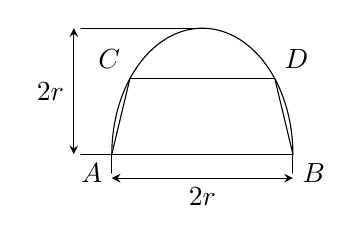
\begin{tikzpicture}[x=1.15cm,y=0.8cm,line join=round,line cap=round,>=stealth]
  \coordinate (A) at (-1,0);
  \coordinate (B) at (1,0);
  \coordinate (C) at (-0.8,1.2);
  \coordinate (D) at (0.8,1.2);
  \draw[domain=180:0,samples=100,smooth,variable=\t] plot ({cos(\t)},{2*sin(\t)});
  \draw (A)--(B);
  \draw (C)--(D);
  \draw (A)--(C);
  \draw (B)--(D);
  \draw[<->] (-1,-0.38)--(1,-0.38) node[midway,below] {$2r$};
  \draw (-1,0)--(-1,-0.30);
  \draw (1,0)--(1,-0.30);
  \draw[<->] (-1.42,0)--(-1.42,2) node[midway,left] {$2r$};
  \draw (-1,0)--(-1.34,0);
  \draw (0,2)--(-1.34,2);
  \node[below left] at (A) {$A$};
  \node[below right] at (B) {$B$};
  \node[above left] at (C) {$C$};
  \node[above right] at (D) {$D$};
\end{tikzpicture}
\end{center}
